\documentclass[11pt,a4paper]{article}
\usepackage[utf8]{inputenc}
\usepackage[english]{babel}
\usepackage{amsmath}
\usepackage{amsfonts}
\usepackage{amssymb}
\usepackage{graphicx}
\graphicspath{{../figures/}}
\author{Jacob Heden Malm}
\title{DD2424 Assignment 4}
\begin{document}
\maketitle

\section{Analytic gradient computations}

Since I wrote my code in python I could not use the provided ComputeGradsNum() method. Instead I performed a sanity check by attempting to over fit my network to a small amount of training examples and monitoring the development of the loss value. I wrote a method called sanity\_check() where I passed in only the first sequence of data points and attempted to get my loss values as low as possible. I trained my network on this data set for 1000 iterations with the standard m and eta parameter settings.\\

Here is an example of the development of the loss values through training on this very limited data set.

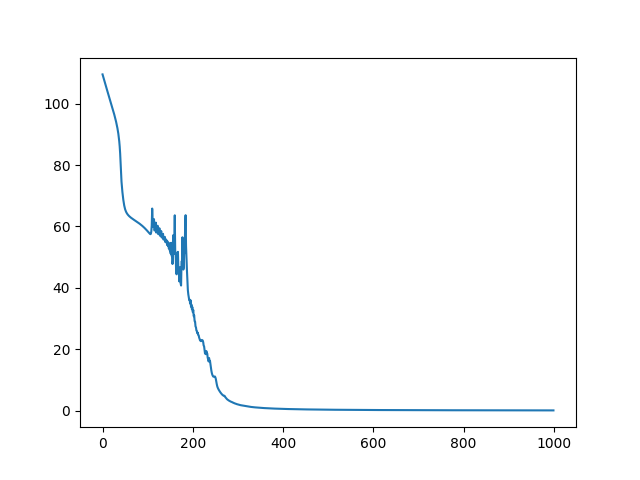
\includegraphics[width=\textwidth]{sanity_check.png}

As we can see, within 1000 iterations the loss goes from roughly 100 to very close to 0, this would not be possible if we did not successfully implement the gradient calculations for all parameters.



\end{document}
